% Provenance (never printed): old seconde/premiere S material on soil as a
% slowly renewed resource (alteration of rocks, clays, the clay--humus
% complex, soil erosion); see sources/book2/PROVENANCE.md. Rates are the
% medians of Montgomery (2007), computed in figdata/grade-10/soil_rates.py.
\chapter{Le sol, une ressource lente à se former}\label{ch:g10:soil-formation}

Une route taillée dans une colline des tropiques humides montre une paroi
de terre rouge, haute de plusieurs fois la taille d'un homme. À son pied, la
roche est encore reconnaissable~: pâle, striée, mais si tendre qu'elle
s'effrite entre les doigts tout en montrant encore les grains et les bandes
de la roche qu'elle a été. Vers le haut, elle passe à une argile bariolée,
puis à une couche rouge et dure, puis à un sol mince où se trouvent les
racines. Toute la paroi était autrefois de la roche massive~: c'est la
roche elle-même, lentement transformée sur place par l'eau et l'air. Le
sol, où poussent toutes les plantes des terres émergées et la nourriture de
presque toute l'humanité, est le sommet d'une telle colonne. Ce chapitre
explique comment la roche devient sol, quelle chimie fait le travail,
comment le climat en règle le rythme, et pourquoi le sol, si lent à se
former, peut se perdre si vite.

\begin{omfigure}
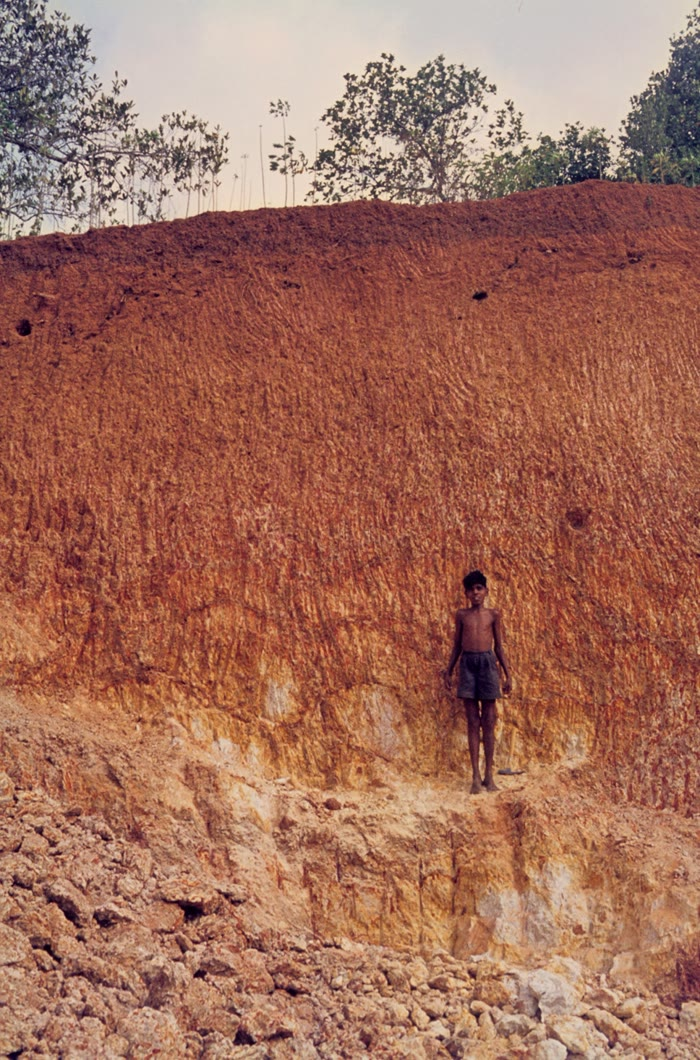
\includegraphics[height=8.5cm]{images/book2/g10-laterite-kerala.jpg}

{\small Un profil d'altération sur un gneiss granitique au Kerala, dans le
sud de l'Inde~: en bas, une roche décomposée et bariolée~; au-dessus, une
\omterm{def:g10:soil-formation:laterite}{latérite} brune, faiblement durcie, sous un sol mince. Le garçon donne
l'échelle. Photographie~: Werner Schellmann, 1969 (CC~BY-SA~2.5).}
\end{omfigure}

\begin{recall}
L'altération fragmente les roches sur place~; l'érosion emporte les
morceaux~; le dépôt les dépose ailleurs (livre~1, année~5). Les roches sont
faites de minéraux, comme le quartz, les feldspaths et les micas d'un
granite (livre~1, année~6). Un sol est une couche vivante faite de grains
minéraux, d'humus, d'eau, d'air et d'organismes~; les décomposeurs
transforment la matière morte en humus~; on décrit un sol par ses couches,
ou horizons (les livres de biologie). Dans une oxydation, une substance perd
des électrons, souvent en se combinant au dioxygène (les livres de chimie).
\end{recall}

\section{De la roche au sol}

L'altération physique --- gélifraction, alternance d'échauffement et de
refroidissement, racines --- fragmente la roche sans changer ses minéraux.
L'\omterm{def:g10:soil-formation:chemical-weathering}{altération chimique} transforme les minéraux eux-mêmes. Ensemble, sur de
longues durées, elles changent le sommet de la roche massive en un manteau
meuble qui s'épaissit vers le bas à mesure que l'altération ronge la roche
sous-jacente.

\begin{definition}[Roche mère~; saprolite]\label{def:g10:soil-formation:weathering-profile}
La \emph{roche mère}\index{roche mere@roche mère} d'un sol est la roche à
partir de laquelle sa partie minérale s'est formée. La
\emph{saprolite}\index{saprolite} est une roche décomposée sur place par
l'altération~: tendre et terreuse, elle montre encore les grains et la
structure de la roche mère. Un \emph{profil d'altération} est la colonne
entière, de la roche saine jusqu'au sol au sommet, en passant par la
saprolite.
\end{definition}
% ledger: usgs:saprolite

La \omterm{def:g10:soil-formation:weathering-profile}{saprolite} peut être épaisse. Sous les collines ondulées qui bordent le
versant est des Appalaches, dans l'est des États-Unis, elle atteint par
endroits environ \qty{46}{m} (150~pieds), même si son épaisseur varie
beaucoup d'un lieu à l'autre~; le sol n'en est que la partie supérieure.
% ledger: usgs:saprolite

\begin{omfigure}
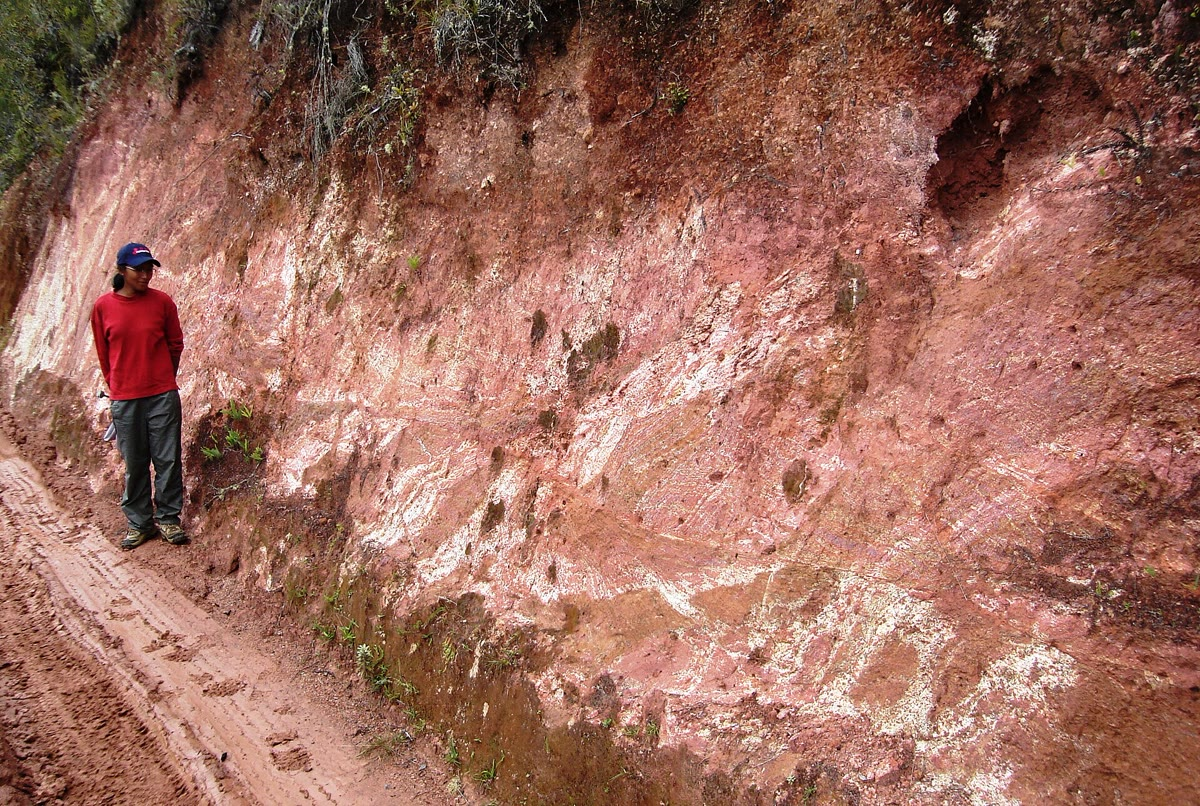
\includegraphics[width=0.8\linewidth]{images/book2/g10-saprolite-madagascar.jpg}

{\small De la \omterm{def:g10:soil-formation:weathering-profile}{saprolite} dans une tranchée routière du centre de
Madagascar~: l'ancien gneiss, décomposé sur place, montre encore ses bandes,
sous forme de traînées d'argile blanche dans une terre rouge.
Photographie~: Diorit (CC~BY-SA~3.0).}
\end{omfigure}

\begin{omfigure}
\begin{tikzpicture}[font=\footnotesize]
  % humid tropical column
  \begin{scope}
    \fill[omThm!45!brown!60] (0,5.4) rectangle (1.8,6.0);
    \fill[omThm!70!orange!70] (0,4.2) rectangle (1.8,5.4);
    \fill[omThm!25!orange!35] (0,1.2) rectangle (1.8,4.2);
    \foreach \y in {1.5,2.1,2.7,3.3,3.9} \draw[white!80!black, thick] (0.1,\y) -- (1.7,\y+0.15);
    \fill[black!30] (0,0) rectangle (1.8,1.2);
    \foreach \x/\y in {0.3/0.3,0.9/0.7,1.4/0.2,0.5/0.9,1.2/1.0} \draw[black!55] (\x,\y) -- ++(0.2,0.08);
    \draw[black!60] (0,0) rectangle (1.8,6.0);
    \node[anchor=north, align=center] at (0.9,-0.1) {tropiques humides};
  \end{scope}
  % temperate column
  \begin{scope}[xshift=3.2cm]
    \fill[omThm!45!brown!60] (0,2.2) rectangle (1.8,2.6);
    \fill[omThm!25!orange!35] (0,1.2) rectangle (1.8,2.2);
    \foreach \y in {1.5,1.9} \draw[white!80!black, thick] (0.1,\y) -- (1.7,\y+0.15);
    \fill[black!30] (0,0) rectangle (1.8,1.2);
    \foreach \x/\y in {0.3/0.3,0.9/0.7,1.4/0.2,0.5/0.9,1.2/1.0} \draw[black!55] (\x,\y) -- ++(0.2,0.08);
    \draw[black!60] (0,0) rectangle (1.8,2.6);
    \node[anchor=north, align=center] at (0.9,-0.1) {climat\\tempéré};
  \end{scope}
  % labels
  \draw[black!50] (5.3,5.7) -- (2.0,5.7); \node[anchor=west] at (5.4,5.7) {sol};
  \draw[black!50] (5.3,4.8) -- (2.0,4.8); \node[anchor=west, align=left] at (5.4,4.8) {latérite~: rouge, riche en oxydes\\de fer et d'aluminium};
  \draw[black!50] (5.3,3.4) -- (2.0,3.4); \node[anchor=west, align=left] at (5.4,3.4) {saprolite~: roche décomposée\\sur place, structure conservée};
  \draw[black!50] (5.3,0.6) -- (5.0,0.6); \node[anchor=west] at (5.4,0.6) {roche mère saine};
\end{tikzpicture}

{\small Deux profils d'altération sur la même roche (schéma, sans
échelle)~: sous un climat chaud et humide, le profil est bien plus épais et
son sommet est une \omterm{def:g10:soil-formation:laterite}{latérite}~; sous un climat tempéré, une \omterm{def:g10:soil-formation:weathering-profile}{saprolite} plus
mince porte le sol.}
\end{omfigure}

\section{L'altération chimique}

\begin{definition}[Altération chimique]\label{def:g10:soil-formation:chemical-weathering}
L'\emph{altération chimique}\index{alteration chimique@altération chimique}
est la transformation des minéraux d'une roche par des réactions avec l'eau
et avec les gaz qu'elle transporte, le dioxyde de carbone et le
dioxygène~: certains minéraux se dissolvent, d'autres sont changés en
nouveaux minéraux, stables à la surface de la Terre.
\end{definition}

L'eau de pluie dissout un peu de dioxyde de carbone de l'air, et bien
davantage en s'infiltrant dans le sol, où les racines et les décomposeurs
le rejettent en respirant. Une partie du gaz dissous forme de l'acide
carbonique, qui libère des ions hydrogène~:
\begin{center}
\ce{CO2 + H2O -> H+ + HCO3-}
\end{center}
Ces ions hydrogène attaquent les minéraux.

\begin{definition}[Hydrolyse]\label{def:g10:soil-formation:hydrolysis}
L'\emph{hydrolyse}\index{hydrolyse} est l'\omterm{def:g10:soil-formation:chemical-weathering}{altération chimique} d'un minéral
silicaté par l'eau et ses ions hydrogène~: les ions hydrogène prennent la
place des ions métalliques du minéral, qui passent en solution, et le reste
du minéral est reconstruit en un \omterm{def:g10:soil-formation:clay}{minéral argileux}.
\end{definition}

\begin{proposition}[Hydrolyse d'un feldspath]\label{prop:g10:soil-formation:hydrolysis}
Le feldspath potassique orthose, \ce{KAlSi3O8}, est transformé par
\omterm{def:g10:soil-formation:hydrolysis}{hydrolyse} en un \omterm{def:g10:soil-formation:clay}{minéral argileux}, la kaolinite, \ce{Al2Si2O5(OH)4}~; les
ions potassium et la silice dissoute, \ce{H4SiO4}, sont emportés par
l'eau~:
\begin{center}
\ce{2 KAlSi3O8 + 2 H+ + 9 H2O -> Al2Si2O5(OH)4 + 2 K+ + 4 H4SiO4}
\end{center}
\end{proposition}
% ledger: webmineral:formulas

\begin{proof}[Vérification]
Compter chaque élément des deux côtés. Potassium~: 2 et 2. Aluminium~: 2
et 2. Silicium~: 6 et $2 + 4 = 6$. Oxygène~: $16 + 9 = 25$ et $9 + 16 = 25$.
Hydrogène~: $2 + 18 = 20$ et $4 + 16 = 20$. Charge~: $+2$ et $+2$.
\end{proof}

\begin{proposition}[Dissolution de la calcite]\label{prop:g10:soil-formation:calcite}
La calcite, \ce{CaCO3}, le minéral du calcaire, se dissout entièrement dans
une eau chargée de dioxyde de carbone~; il ne reste rien de solide~:
\begin{center}
\ce{CaCO3 + CO2 + H2O -> Ca^2+ + 2 HCO3-}
\end{center}
\end{proposition}
% ledger: webmineral:formulas

Le fer est attaqué d'une troisième façon. Dans les minéraux sombres d'une
roche, comme le mica noir d'un granite, le fer est sous la forme réduite
\ce{Fe^2+}. Le dioxygène apporté par l'eau l'oxyde, et le fer(III) reste sur
place sous forme d'oxydes insolubles~: la goethite jaune-brun, \ce{FeO(OH)},
et l'hématite rouge, \ce{Fe2O3}. Pour la goethite~:
\begin{center}
\ce{4 Fe^2+ + O2 + 6 H2O -> 4 FeO(OH) + 8 H+}
\end{center}
Ces oxydes colorent en jaune, en brun et en rouge les roches altérées et les
sols.
% ledger: webmineral:formulas

Tous les minéraux ne s'altèrent pas au même rythme. Dans un granite qui
s'altère, le mica noir rouille et les feldspaths se changent en argile, mais
les grains de quartz, presque insolubles, en sortent intacts~: ils finissent
en sable.

\begin{example}[L'altération d'un granite]\label{ex:g10:soil-formation:granite}
% ledger: webmineral:formulas (masses computed in figdata/grade-10/soil_rates.py)
Un kilogramme d'orthose contient $1000/278.33 \approx \qty{3.59}{mol}$ de
\ce{KAlSi3O8}. D'après l'équation, deux moles d'orthose donnent une mole de
kaolinite~: $3.59/2 \approx \qty{1.80}{mol}$, soit $1.80 \times 258.16
\approx \qty{464}{g}$ d'argile. Le potassium, $14.05~\%$ de la masse de
l'orthose, soit \qty{140.5}{g}, et $2 \times 3.59 = \qty{7.19}{mol}$ de
silice partent en solution. D'un granite fait de quartz, de feldspaths et
de micas, l'altération laisse du sable (le quartz), de l'argile (issue des
feldspaths et des micas) et des oxydes de fer, et envoie aux rivières le
potassium, le sodium, le calcium et la silice.
\end{example}

\section{Argiles et humus}

\begin{definition}[Minéral argileux]\label{def:g10:soil-formation:clay}
Un \emph{minéral argileux}\index{mineral argileux@minéral argileux} est un
silicate fait de minces feuillets d'atomes empilés les uns sur les autres,
formé par l'altération, qui se présente en paillettes bien plus petites que
des grains de sable. La kaolinite en est un.
\end{definition}
% ledger: webmineral:formulas

Les surfaces des paillettes d'argile portent des charges électriques
négatives. Elles retiennent des ions positifs --- potassium \ce{K+}, calcium
\ce{Ca^2+}, magnésium \ce{Mg^2+}, ammonium \ce{NH4+} --- que la pluie
emporterait sinon. L'humus fait de même. Liés ensemble, l'argile et l'humus
forment le \emph{complexe argilo-humique}, la réserve de sels minéraux
nutritifs du sol~: une racine libère des ions hydrogène et prend en échange
le potassium ou le calcium retenus sur les paillettes.

\begin{omfigure}
\begin{tikzpicture}[font=\footnotesize, >={Stealth[length=2mm]}]
  \foreach \y in {0,0.7,1.4} {
    \fill[omExo!35, draw=black!60] (0,\y) rectangle (7.2,\y+0.3);
    \foreach \x in {0.3,0.9,...,7.0} \node[font=\tiny, black!70] at (\x,\y+0.15) {$-$};
  }
  \foreach \x/\ion in {0.7/K^+, 1.9/Ca^{2+}, 3.1/K^+, 4.3/Mg^{2+}, 5.5/NH_4^+, 6.7/K^+} {
    \fill[omThm!20, draw=omThm!80!black] (\x,2.1) circle (0.4);
    \node[font=\scriptsize] at (\x,2.1) {$\mathrm{\ion}$};
  }
  \foreach \x in {1.3, 3.7, 6.1} \fill[omThm!20, draw=omThm!80!black] (\x,0.5) circle (0.17);
  \foreach \x in {2.5, 4.9} \fill[omThm!20, draw=omThm!80!black] (\x,1.2) circle (0.17);
  \node[anchor=north] at (3.6,-0.1) {feuillets d'argile chargés négativement, avec des ions positifs entre eux};
  \node[anchor=south] at (3.1,2.5) {ions positifs retenus sur les surfaces};
  % root and exchange
  \draw[line width=2.2pt, brown!60!black] (9.6,3.4) .. controls (9.3,2.6) and (8.9,2.2) .. (8.1,2.0);
  \node[anchor=east] at (9.25,3.3) {racine};
  \draw[->, omDef!80!black, thick] (8.0,2.2) .. controls (7.6,2.6) and (7.2,2.6) .. (6.95,2.3);
  \node[anchor=south, omDef!80!black] at (7.5,2.55) {\ce{H+} cédé};
  \draw[->, omThm!80!black, thick] (6.95,1.8) .. controls (7.3,1.5) and (7.7,1.6) .. (8.0,1.85);
  \node[anchor=north, omThm!80!black] at (7.8,1.55) {\ce{K+} prélevé};
\end{tikzpicture}

{\small Le complexe argilo-humique (schéma)~: les feuillets d'argile chargés
négativement retiennent des ions positifs à leur surface et entre eux~; une
racine échange des ions hydrogène contre ces éléments nutritifs.}
\end{omfigure}

\section{Les sols et le climat}

L'\omterm{def:g10:soil-formation:chemical-weathering}{altération chimique} a besoin d'eau et, comme la plupart des réactions,
elle est plus rapide quand il fait chaud. Là où le climat est à la fois
chaud et humide, la roche se décompose le plus profondément et le plus
complètement~: les feldspaths se changent entièrement en argile, une grande
partie de la silice elle-même est emportée, et ce qui reste est riche en
éléments les moins solubles, le fer et l'aluminium.

\begin{definition}[Latérite]\label{def:g10:soil-formation:laterite}
Une \emph{latérite}\index{laterite@latérite} est un matériau profondément
altéré des climats chauds et humides, rouge ou brun, fait surtout d'oxydes
de fer et d'aluminium et de kaolinite, dont presque tout ce qui est soluble
a été retiré.
\end{definition}

Sous les climats froids, gelés une grande partie de l'année, et sous les
climats secs, où l'eau est rare, l'\omterm{def:g10:soil-formation:chemical-weathering}{altération chimique} est lente~: les sols
sont minces et la roche se trouve juste en dessous. Des pôles à l'équateur,
la profondeur d'altération est la plus grande sous les forêts tropicales
humides et la plus faible dans les déserts et les régions polaires.

\begin{omfigure}
\begin{tikzpicture}[font=\footnotesize]
  \fill[black!25] (0,-0.2) -- (0,-0.5) .. controls (1.5,-0.6) and (2.5,-1.4) .. (3.4,-1.2)
     .. controls (4.2,-1.0) and (4.6,-0.55) .. (5.2,-0.5) .. controls (6.0,-0.5) and (6.6,-1.6) .. (7.6,-3.0)
     .. controls (8.2,-3.6) and (9.0,-3.6) .. (10,-3.4) -- (10,-3.8) -- (0,-3.8) -- cycle;
  \fill[omThm!25!orange!35] (0,0) -- (10,0) -- (10,-3.4) .. controls (9.0,-3.6) and (8.2,-3.6) .. (7.6,-3.0)
     .. controls (6.6,-1.6) and (6.0,-0.5) .. (5.2,-0.5) .. controls (4.6,-0.55) and (4.2,-1.0) .. (3.4,-1.2)
     .. controls (2.5,-1.4) and (1.5,-0.6) .. (0,-0.5) -- cycle;
  \draw[black!60] (0,0) -- (10,0);
  \node[anchor=south] at (0.6,0.05) {polaire};
  \node[anchor=south] at (3.2,0.05) {tempéré};
  \node[anchor=south] at (5.3,0.05) {désert};
  \node[anchor=south] at (6.8,0.05) {savane};
  \node[anchor=south] at (9.0,0.05) {forêt tropicale};
  \node[anchor=north] at (0.4,-3.85) {pôle};
  \node[anchor=north] at (9.6,-3.85) {équateur};
  \node[black!70] at (2.0,-2.6) {roche saine};
  \node[black!80] at (8.35,-1.0) {roche altérée et sol};
\end{tikzpicture}

{\small La profondeur d'altération d'un pôle à l'équateur (schéma,
profondeurs sans échelle)~: faible sous les climats polaires et
désertiques, moyenne sous les climats tempérés, maximale sous les forêts
tropicales humides.}
\end{omfigure}

\section{Lent à se former, prompt à se perdre}

À quelle vitesse le sol se forme-t-il~? La production de sol, le rythme
auquel l'altération change la roche en sol à la base du profil, a été
mesurée en de nombreux sites du monde, tout comme le rythme auquel le sol
est érodé en surface. Une compilation de ces mesures donne les vitesses
typiques (médianes) ci-dessous, chacune exprimée en épaisseur de sol par
an.
% ledger: montgomery:rates

\begin{omfigure}
\begin{tikzpicture}
\begin{axis}[omrecord, width=0.82\linewidth, height=5.6cm, ymode=log, log origin=infty, ymin=0.005,
  ymax=5, ybar, bar width=16pt, xtick={0,1,2,3,4}, xmin=-0.6, xmax=4.6,
  xticklabels={{production\\de sol}, {érosion sous\\végétation naturelle}, {érosion\\géologique}, {agriculture\\de conservation}, {labour\\conventionnel}},
  xticklabel style={align=center, font=\scriptsize},
  ylabel={vitesse (\unit{mm} par an)}, tick label style={font=\small}, label style={font=\small},
  nodes near coords, nodes near coords style={font=\scriptsize}, point meta=explicit symbolic]
\addplot[fill=omDef!45, draw=omDef!80!black] table[x=idx, y=rate_mm_yr, meta=rate_mm_yr] {figdata/out/grade-10-soil_rates-rates.dat};
\end{axis}
\end{tikzpicture}

{\small Vitesses médianes de production de sol et d'érosion, d'après une
compilation mondiale de mesures, en millimètres de sol par an (échelle
logarithmique~: chaque graduation vaut dix fois la précédente).
Données~: Montgomery (2007), \emph{Proceedings of the National Academy of
Sciences}.}
\end{omfigure}
% ledger: montgomery:rates

Sous la végétation naturelle, le sol est érodé à peu près aussi vite qu'il
se forme, environ \qty{0.02}{mm} par an~: un centimètre en quelque six
siècles. Sous un labour conventionnel, qui laisse le sol nu entre les
cultures, la vitesse médiane d'érosion est de \qty{1.5}{mm} par an,
quatre-vingt-dix fois la vitesse de production de sol. Sous une agriculture
de conservation, qui perturbe moins le sol et le garde couvert, la médiane
tombe à \qty{0.08}{mm} par an, bien plus près de la vitesse de production.
% ledger: montgomery:rates (ratios computed in figdata/grade-10/soil_rates.py)

\begin{method}[Comparer une vitesse de formation et une vitesse d'érosion]\label{met:g10:soil-formation:rates}
\begin{enumerate}
  \item Exprimer les deux vitesses dans la même unité (millimètres par an).
  \item La perte nette est la vitesse d'érosion $E$ moins la vitesse de
        production $P$.
  \item Un sol d'épaisseur $S$ est perdu en $T = S/(E - P)$ ans~; si
        $E \le P$, le sol ne se perd pas.
  \item Former une épaisseur $S$ à partir de rien demande $S/P$ ans.
\end{enumerate}
\end{method}
% ledger: montgomery:lifetime

Avec ces vitesses, un mètre de sol met environ $1000/0.017 \approx 59\,000$
ans à se former, et sous un labour conventionnel il peut être perdu en
environ
$1000/(1.537 - 0.017) \approx 660$ ans. À l'échelle humaine, le sol est une
ressource qui ne se renouvelle pas.
% ledger: montgomery:rates, montgomery:lifetime

\begin{omfigure}
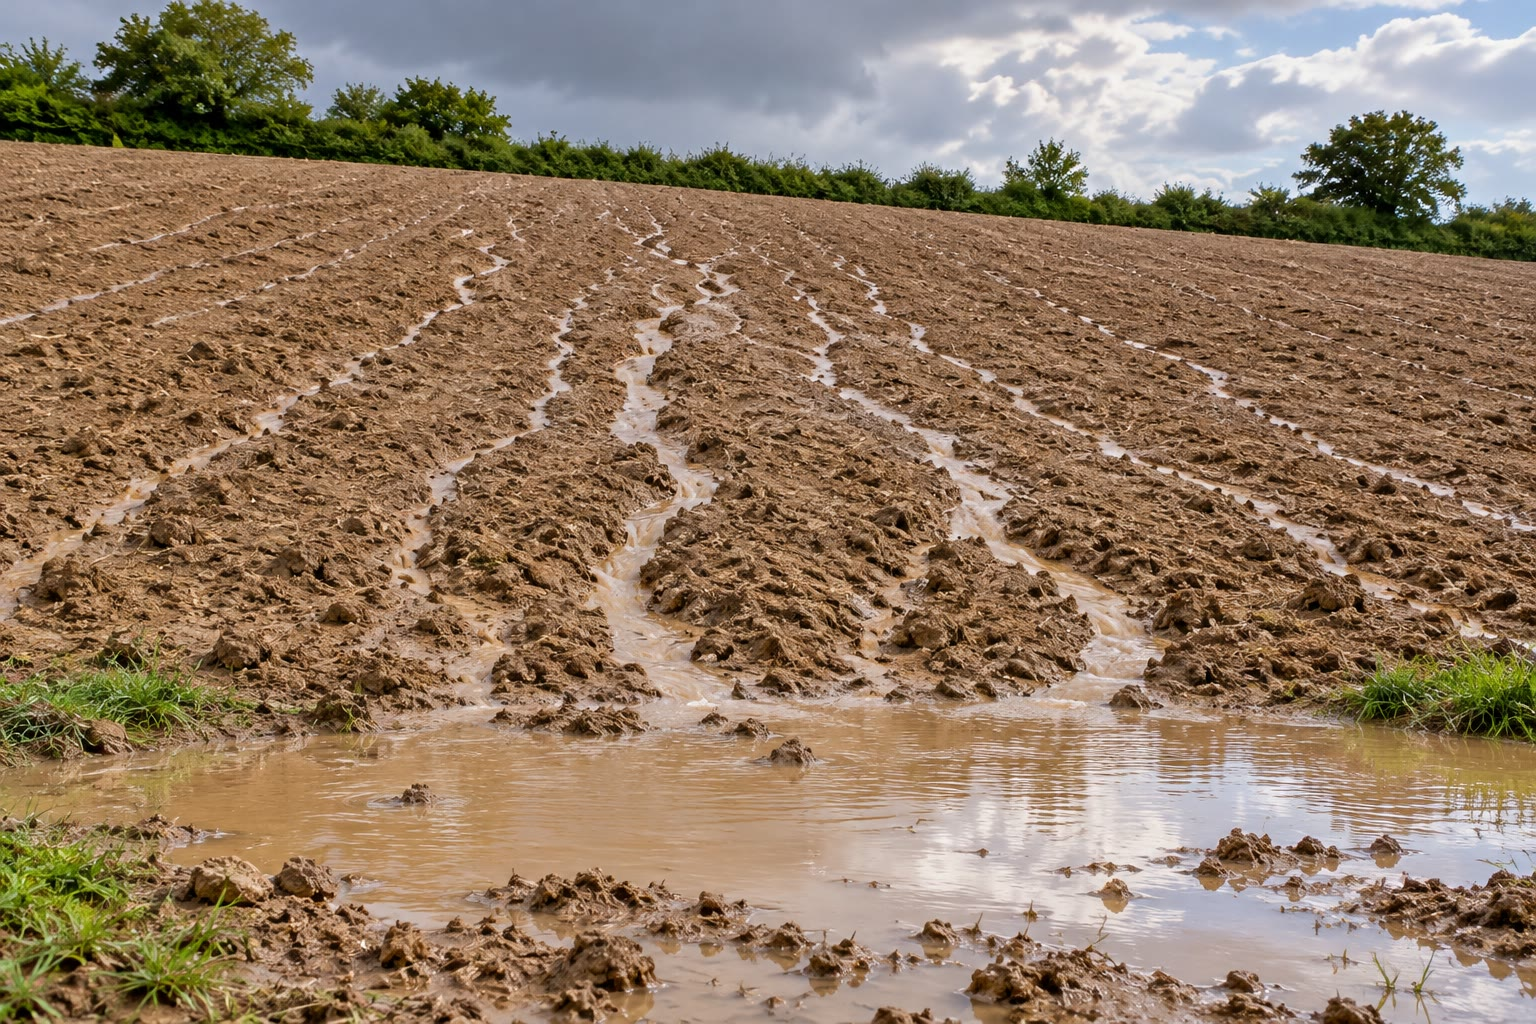
\includegraphics[width=0.72\linewidth]{images/book2/ai/g10-ploughed-rills.jpg}

{\small Un champ labouré après un violent orage~: le ruissellement a creusé
de petits chenaux, ou rigoles, dans le sens de la pente et a emporté le sol
dans une mare boueuse à son pied.}
\end{omfigure}

\section{Exercices}

\begin{exercise}[$\star$]\label{exo:g10:soil-formation:1}
Définir l'\omterm{def:g10:soil-formation:chemical-weathering}{altération chimique} et l'\omterm{def:g10:soil-formation:hydrolysis}{hydrolyse}.
\end{exercise}

\begin{exercise}[$\star$]\label{exo:g10:soil-formation:2}
Qu'est-ce que la \omterm{def:g10:soil-formation:weathering-profile}{saprolite}~? Comment distinguer une \omterm{def:g10:soil-formation:weathering-profile}{saprolite} d'un sol formé
dans du sable apporté par une rivière~?
\end{exercise}

\begin{exercise}[$\star$]\label{exo:g10:soil-formation:3}
Nommer les produits de l'altération d'un granite~: que devient chacun de ses
trois minéraux principaux~?
\end{exercise}

\begin{exercise}[$\star$]\label{exo:g10:soil-formation:4}
Pourquoi les roches altérées et les sols tropicaux sont-ils si souvent
rouges, jaunes ou bruns~?
\end{exercise}

\begin{exercise}[$\star$]\label{exo:g10:soil-formation:5}
À l'aide du diagramme en barres, donner la vitesse médiane de production de
sol et la vitesse médiane d'érosion sous un labour conventionnel. Combien de
fois la seconde est-elle plus grande~?
\end{exercise}

\begin{exercise}[$\star\star$]\label{exo:g10:soil-formation:6}
Vérifier que l'équation de la dissolution de la calcite est équilibrée,
pour chaque élément et pour la charge.
\end{exercise}

\begin{exercise}[$\star\star$]\label{exo:g10:soil-formation:7}
Le calcaire se dissout entièrement, le granite laisse du sable et de
l'argile. Expliquer la différence à l'aide des deux réactions du chapitre.
\end{exercise}

\begin{exercise}[$\star\star$]\label{exo:g10:soil-formation:8}
Expliquer comment le complexe argilo-humique retient le potassium dans un
sol que la pluie traverse, et comment une racine le prélève.
\end{exercise}

\begin{exercise}[$\star\star$]\label{exo:g10:soil-formation:9}
Donner deux raisons pour lesquelles les \omterm{def:g10:soil-formation:laterite}{latérites} se forment sous les
climats chauds et humides et non sous les climats froids ou secs.
\end{exercise}

\begin{exercise}[$\star\star$]\label{exo:g10:soil-formation:10}
La vitesse médiane de production de sol est de \qty{0.017}{mm} par an.
Combien de temps faut-il pour former \qty{1}{cm}, \qty{30}{cm} et \qty{1}{m}
de sol~?
\end{exercise}

\begin{exercise}[$\star\star$]\label{exo:g10:soil-formation:11}
Les vitesses d'érosion sont souvent données en masse de sol par hectare et
par an. Avec une masse volumique du sol de \qty{1200}{kg/m^3}, quelle masse
représente une perte de \qty{1.5}{mm} par an sur un hectare
(\qty{10000}{m^2})~?
\end{exercise}

\begin{exercise}[$\star\star\star$]\label{exo:g10:soil-formation:12}
Une \omterm{def:g10:soil-formation:weathering-profile}{saprolite} de \qty{46}{m} d'épaisseur s'est formée sous les collines
d'une région tempérée. Si l'altération progressait dans la roche à
\qty{0.017}{mm} par an, combien de temps cela aurait-il pris~? Que suggère
la réponse sur l'âge d'un tel paysage~?
\end{exercise}

\begin{exercise}[$\star\star\star$]\label{exo:g10:soil-formation:13}
Écrire l'équation de l'oxydation de \ce{Fe^2+} en goethite donnée dans le
chapitre et la vérifier. Puis écrire et équilibrer l'oxydation de \ce{Fe^2+}
en hématite, \ce{Fe2O3}, par le dioxygène et l'eau, avec libération de
\ce{H+}.
\end{exercise}

\begin{exercise}[$\star\star\star$]\label{exo:g10:soil-formation:14}
Sous une agriculture de conservation, la vitesse médiane d'érosion est de
\qty{0.082}{mm} par an. Avec une production de sol de \qty{0.017}{mm} par
an, combien de temps faut-il pour perdre \qty{30}{cm} de sol~? Comparer au
labour conventionnel.
\end{exercise}

\begin{exercise}[$\star\star\star$]\label{exo:g10:soil-formation:15}
Un granite contient \qty{30}{\percent} d'orthose en masse. Quelle masse de
kaolinite se forme quand une tonne de ce granite a vu toute son orthose
s'altérer, et quelle masse de potassium est libérée~?
\end{exercise}

\section{Problème~: la durée de vie d'un sol}

\begin{problem}[{Problème du week-end --- de la roche au champ, et retour à la rivière}]
\label{pb:g10:soil-formation:1}
% ledger: montgomery:rates, montgomery:lifetime, webmineral:formulas (values computed in figdata/grade-10/soil_rates.py)

\begin{center}
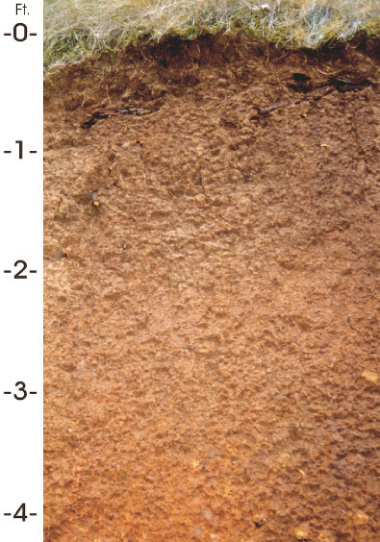
\includegraphics[height=6cm]{images/book2/g10-nrcs-jory-soil.jpg}

{\small Un profil de sol, avec une échelle en pieds à gauche (\num{1}~pied =
\qty{0.3048}{m}). Photographie~: USDA Natural Resources Conservation Service
(domaine public).}
\end{center}

\medskip
\noindent\textbf{Partie I --- Un profil.}
\begin{enumerate}
  \item L'échelle atteint 4~pieds près du bas de l'image. Quelle profondeur
        cela représente-t-il, en mètres~?
  \item La couche sombre du sommet descend jusqu'à un demi-pied environ.
        Quelle est son épaisseur, en centimètres~?
  \item Qu'est-ce qui donne à cette couche supérieure sa couleur sombre~?
  \item En dessous, le sol est brun rougeâtre. Quels minéraux lui donnent
        cette couleur, et comment se sont-ils formés~?
  \item La \omterm{def:g10:soil-formation:weathering-profile}{roche mère} est-elle visible sur la photographie~? Que
        s'attendrait-on à trouver sous le bas de l'image~?
\end{enumerate}

\medskip
\noindent\textbf{Partie II --- La chimie d'un granite qui s'altère.}
\begin{enumerate}[resume]
  \item Écrire l'équation de l'\omterm{def:g10:soil-formation:hydrolysis}{hydrolyse} de l'orthose.
  \item Combien de moles d'orthose y a-t-il dans \qty{1}{kg}
        (\qty{278.33}{g/mol})~?
  \item Quelle masse de kaolinite (\qty{258.16}{g/mol}) donnent-elles~?
  \item Qu'est-ce qui part avec l'eau, et où cela va-t-il~?
  \item Que devient le quartz du granite~?
\end{enumerate}

\medskip
\noindent\textbf{Partie III --- Formation contre érosion.}
\begin{enumerate}[resume]
  \item Le sol se forme à \qty{0.017}{mm} par an. Combien de temps faut-il
        pour former le profil de la partie~I~?
  \item Sous un labour conventionnel, le sol est érodé à \qty{1.537}{mm}
        par an. Quelle est la perte nette chaque année~?
  \item Combien de temps durerait le profil de la partie~I~?
  \item Comparer les deux durées des questions 11 et 13.
  \item Sous la végétation naturelle, l'érosion est de \qty{0.013}{mm} par
        an. Le sol se perd-il~?
\end{enumerate}

\medskip
\noindent\textbf{Partie IV --- La durée de vie du sol.}
\begin{enumerate}[resume]
  \item Écrire la durée $T$ nécessaire pour perdre une épaisseur $S$ de sol
        en fonction de $S$, de la vitesse d'érosion $E$ et de la vitesse de
        production $P$.
  \item Calculer $T$ pour $S = \qty{30}{cm}$ sous un labour conventionnel.
  \item Calculer $T$ pour $S = \qty{30}{cm}$ sous une agriculture de
        conservation (\qty{0.082}{mm} par an).
  \item Pourquoi peut-on dire qu'un sol est une ressource qui ne se
        renouvelle pas à l'échelle humaine~?
  \item Combien de temps faut-il pour perdre un mètre de sol sous un labour
        conventionnel~?
\end{enumerate}
\end{problem}
